% !TEX root = ../main.tex
\chapter{Topic Modeling}
\label{ch:topicModeling}

Topic models are probabilistic models which are used to extract an underlying semantic structure from text artifacts, or documents.
They are based on a hierarchical bayesian analysis on the terms in a document,
on which a similarity measure for the its content can be defined and used to "connect" and cluster documents.
\par
Topic models are useful when dealing with large quantities of unstructured documents,
that need to be automatically structured, grouped or filtered for knowledge extraction,
for example to provide similar/related content at the end of blog entries,
or to automatically tag content with relevant keywords~\ref{blei2009topic}.
\par
In this chapter, methods for topic modeling will be explored,
and a suitable model for the use-case of this thesis will be determined.
While it is easy for humans to gain an intuitive understanding what a document is about
and other subjective attributes, machines lack this intuition.
Therefore, the topic modeling methods presented in this chapter infer \textit{latent} topics,
meaning that they are unable to name or describe a topic, but merely confirm its existence.
However, since the topics inferred are dependent on term (in this case: word) frequencies,
the models can provide a human-understandable representation of a topic by listing its most frequent terms.

\section{Methods}
\label{sec:methods_topicmodeling}

Similar to the previous chapter, multiple methods to perform topic modeling will be explained and demonstrated.
However, since no labeled dataset of a representative sample of statuses on Twitter and their respective topics is available,
only subjective assessments can be made to their performance.
Although the Sanders-dataset was collected by filtering a stream for specific keywords as described in~\ref{sec:theSandersDataset},
and these could be used as labels for a supervised approach such as supervised LDA~\ref{Blei2008},
the dataset is not representative of all activity on Twitter and not suitable for training such a model.
Therefore, only unsupervised approaches will be considered,
and subjective choices will be made as to what constitutes a "topic" in the context of this thesis,
with the parameters for the models being determined accordingly.

\subsection{TF-IDF}
\label{subsec:tfidf}

Both algorithms use TF-IDF (\textbf{T}erm \textbf{F}requency - \textbf{I}nverse \textbf{D}ocument \textbf{F}requency).
In the TF-IDF scheme, first, a dictionary of terms (words, usually) that the documents are made of is formed.
In this case, this dictionary will be created by taking all the terms (words) in the dataset,
and removing those that occur only once, to reduce its size.
Also, contrary to~\ref{ch:sentimentAnalysis}, in this chapter,
the tokenization function will also remove stopwords, as described in~\ref{sec:preprocessingAndtermization}.
Another strategy that could've been used for scenarios where comprehensive stopword lists are not available
would be to remove a percentage or absolute number of most and least frequent terms,
which have little informativeness since they occur in too many or too few documents.
The implementation of the dictionary creation process can be seen in~\ref{code:create_corpus}.

\begin{figure}
    \caption{Implementation of corpus-creation}
    \label{code:create_corpus}
    % @formatter:off
    \begin{minted}{python}
        # The usual preprocessing and tokenization
        tweets = [tokenize(preprocess(tweet) for tweet in tweets]

        # Count term occurences
        term_count_dictionary = defaultdict(int)
        for tweet in tweets:
            for term in tweet:
                term_count_dictionary[term] += 1

        # keep terms that occur more than once
        terms = [[(term, term_count_dictionary[term]) for term in tweet if term_count_dictionary[term] > 1] for tweet in tweets]
    \end{minted}
    % @formatter:on
\end{figure}

\par
To compute the TF-IDF values for a specific document,
a term count vector is then formed containing how often each term in the dictionary occurs in that document,
and normalized over the length to result in the frequency.
This is usually sparsely implemented, since especially with short Twitter statuses,
most words in the corpus do not occur in the document.
Also, since some words might generally occur more often, thereby being less informative of the topic,
the frequency for each term in the document is then divided by the frequency of that term in the dictionary,
giving $term frequency / document frequency$, or $term frequency \* inverse document frequency$ (TF-IDF)~\cite{Blei2003}.
\par
The gensim library was used to create and save the TF-IDF model,
which contains rows with two term identifiers (the terms themselves are saved in the dictionary) and a count of how often
they cooccurr in any of the training documents, while omitting term-combinations that never coocurr, to reduce size~\cite{gensimDocs}.

\subsection{LDA}
\label{subsec:lda}

The basic idea behind LDA (\textbf{L}atent \textbf{D}irichlet \textbf{A}llocation) is to represent documents as a distribution of (latent) topics,
each of which is characterized as a distribution over words.
This thesis will provide an outside view of this method, while explaining important hyperparameters and their impact.
LDA is a bag-of-words model, which means there are no syntax rules.
\\
An LDA model takes the TF-IDF model created in~\ref{subsec:tfidf} as an input to determine the dirichlet distributions,
and two major hyperparameters, $\alpha$ and $\eta$,
both of which are parameters of the internal dirichlet-distributions.
\\
$\alpha$ controls the per-document topic dirichlet distribution,
where a higher value indicates that documents tend to be a mixture of many topics,
and lower values lead to few topics with higher probability.
\\
$\eta$ (also sometimes denoted $\beta$) controls the per-topic word dirichlet distribution, where, as with $\alpha$,
higher values lead to few words with high probabilities determining the topics,
and vice-versa.
\\
The output is a matrix where every row represents a topic,
the columns are the terms from the dictionary,
and every element represents the probability that the word belongs to the topic,
with every column therefore adding up to 1.
When classifying a document, this matrix is used to allocate a distribution of topics for which the probability to have generated that document is maximized~\cite{Blei2003}.
\par
%First, try the default settings
For LDA topic modeling, the gensim library was used~\cite{gensimDocs}.
The dataset used was the streaming sample dataset described in~\ref{sec:streamingSampleDataset},
since the Sanders dataset is topically not representative of Twitter, as described in~\ref{sec:theSandersDataset}.

To explore the results and determine the best hyperparameters, LDAvis was used.
LDAvis plots the topics on a 2D-scatterplot, with the axes being the top 2 principal components
in the hyperdimensional space of all topics, to visualize topic similarity and overlap~\cite{}.
It can also list the most relevant terms for each topic showing their frequencies in relation to their overall frequencies,
where relevancy is determined through a formula developed by Sievert \etAl~\cite{sievert2014ldavis},
which can be seen in~\ref{math:relevance}.

\begin{figure}
    \caption{Relevancy measure used in LDAvis, developed by Sievert \etAl~\cite{sievert2014ldavis}}
    \label{math:relevance}
    \begin{align*}
        relevance(term w | topic t) = \lambda \* p(w | t) + (1 - \lambda) \* \frac{p(w | t)}{p(w)}
    \end{align*}
\end{figure}

$\lambda$ adjusts the relative importance of words that are discriminant to a certain topic,
where 0.5 was found to be a good value.

After some exploration, the best-suited hyperparameters were chosen.
The number of topics was set to 10.
$\eta$ was set to 0.01, which also showed good results in previous Twitter topic modeling research~\cite{Hong2010}.
$\alpha$ is set to "auto", which means gensim learns it from the data provided, and proved to give better results than trying around.
The LDAvis visualization for this model can be seen in~\ref{ldavis}.

\begin{figure}
    \centering
    \caption{LDAvis visualization of the topic model trained on the sample dataset.}
    \label{fig:ldavis}
    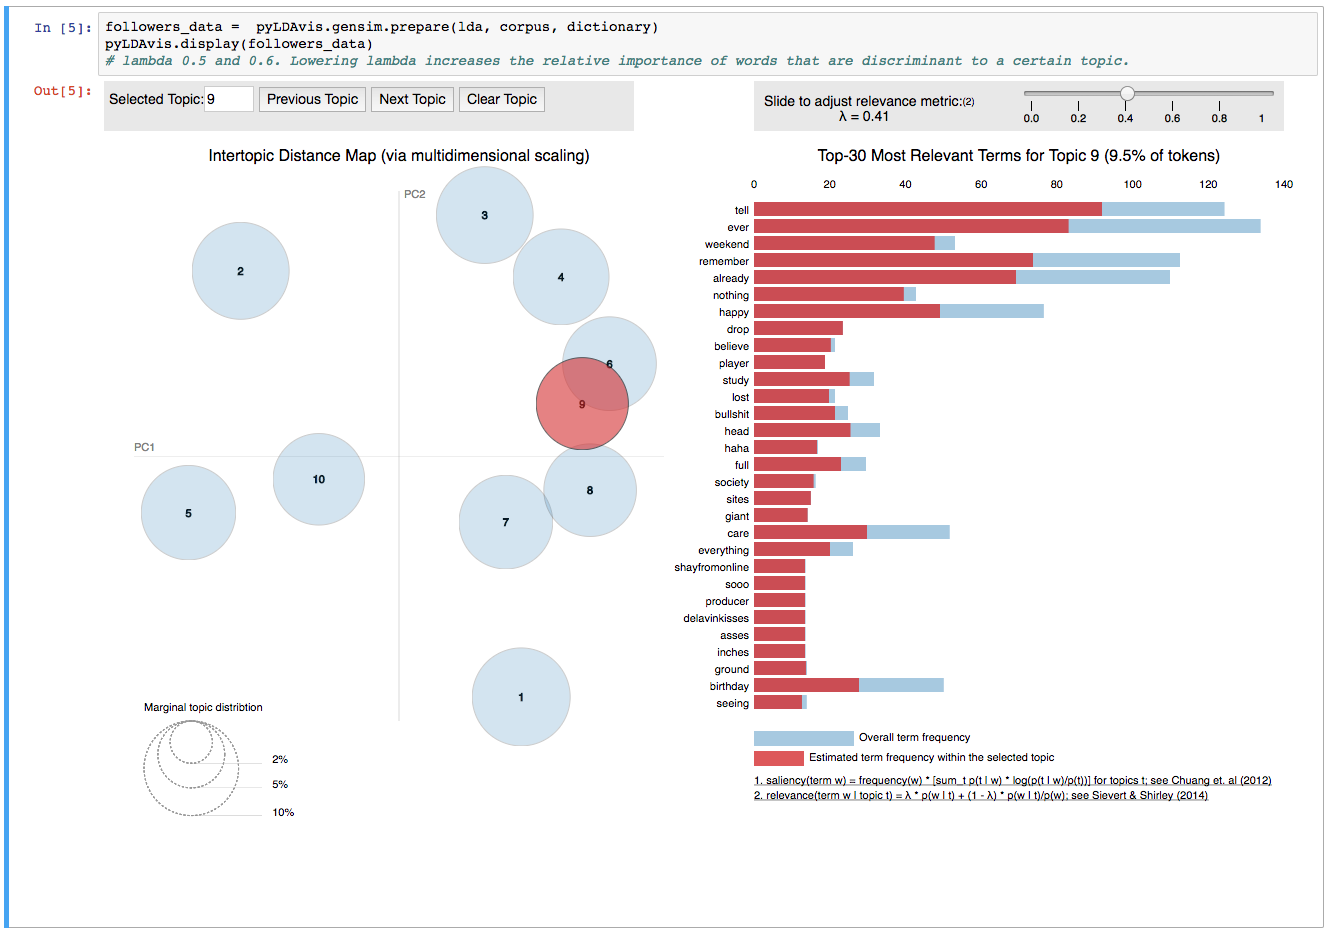
\includegraphics[width=10cm]{../images/LDAvis.png}
\end{figure}

\par
Next, a different visualization, as a network graph, was devised to make a subjective assessment of the model.
In the graph, each light-blue node represents a topic.
For each topic, the 5 terms with the highest probabilities are connected with edges whose weight (thickness) represent the probability
of that word being in a document of that topic, as computed by the model.
It can be seen that some topics share terms - however, these shared terms are not very distinct terms.
The model even successfully modeled trending topics on the evening when the data was collected as described in~\ref{sec:streamingSampleDataset}.
The network graph can be seen in~\ref{fig:lda_network_graph}

\begin{figure}
    \centering
    \caption{Network graph of the LDA topic model created from the stream sample dataset}
    \label{fig:lda_network_graph}
    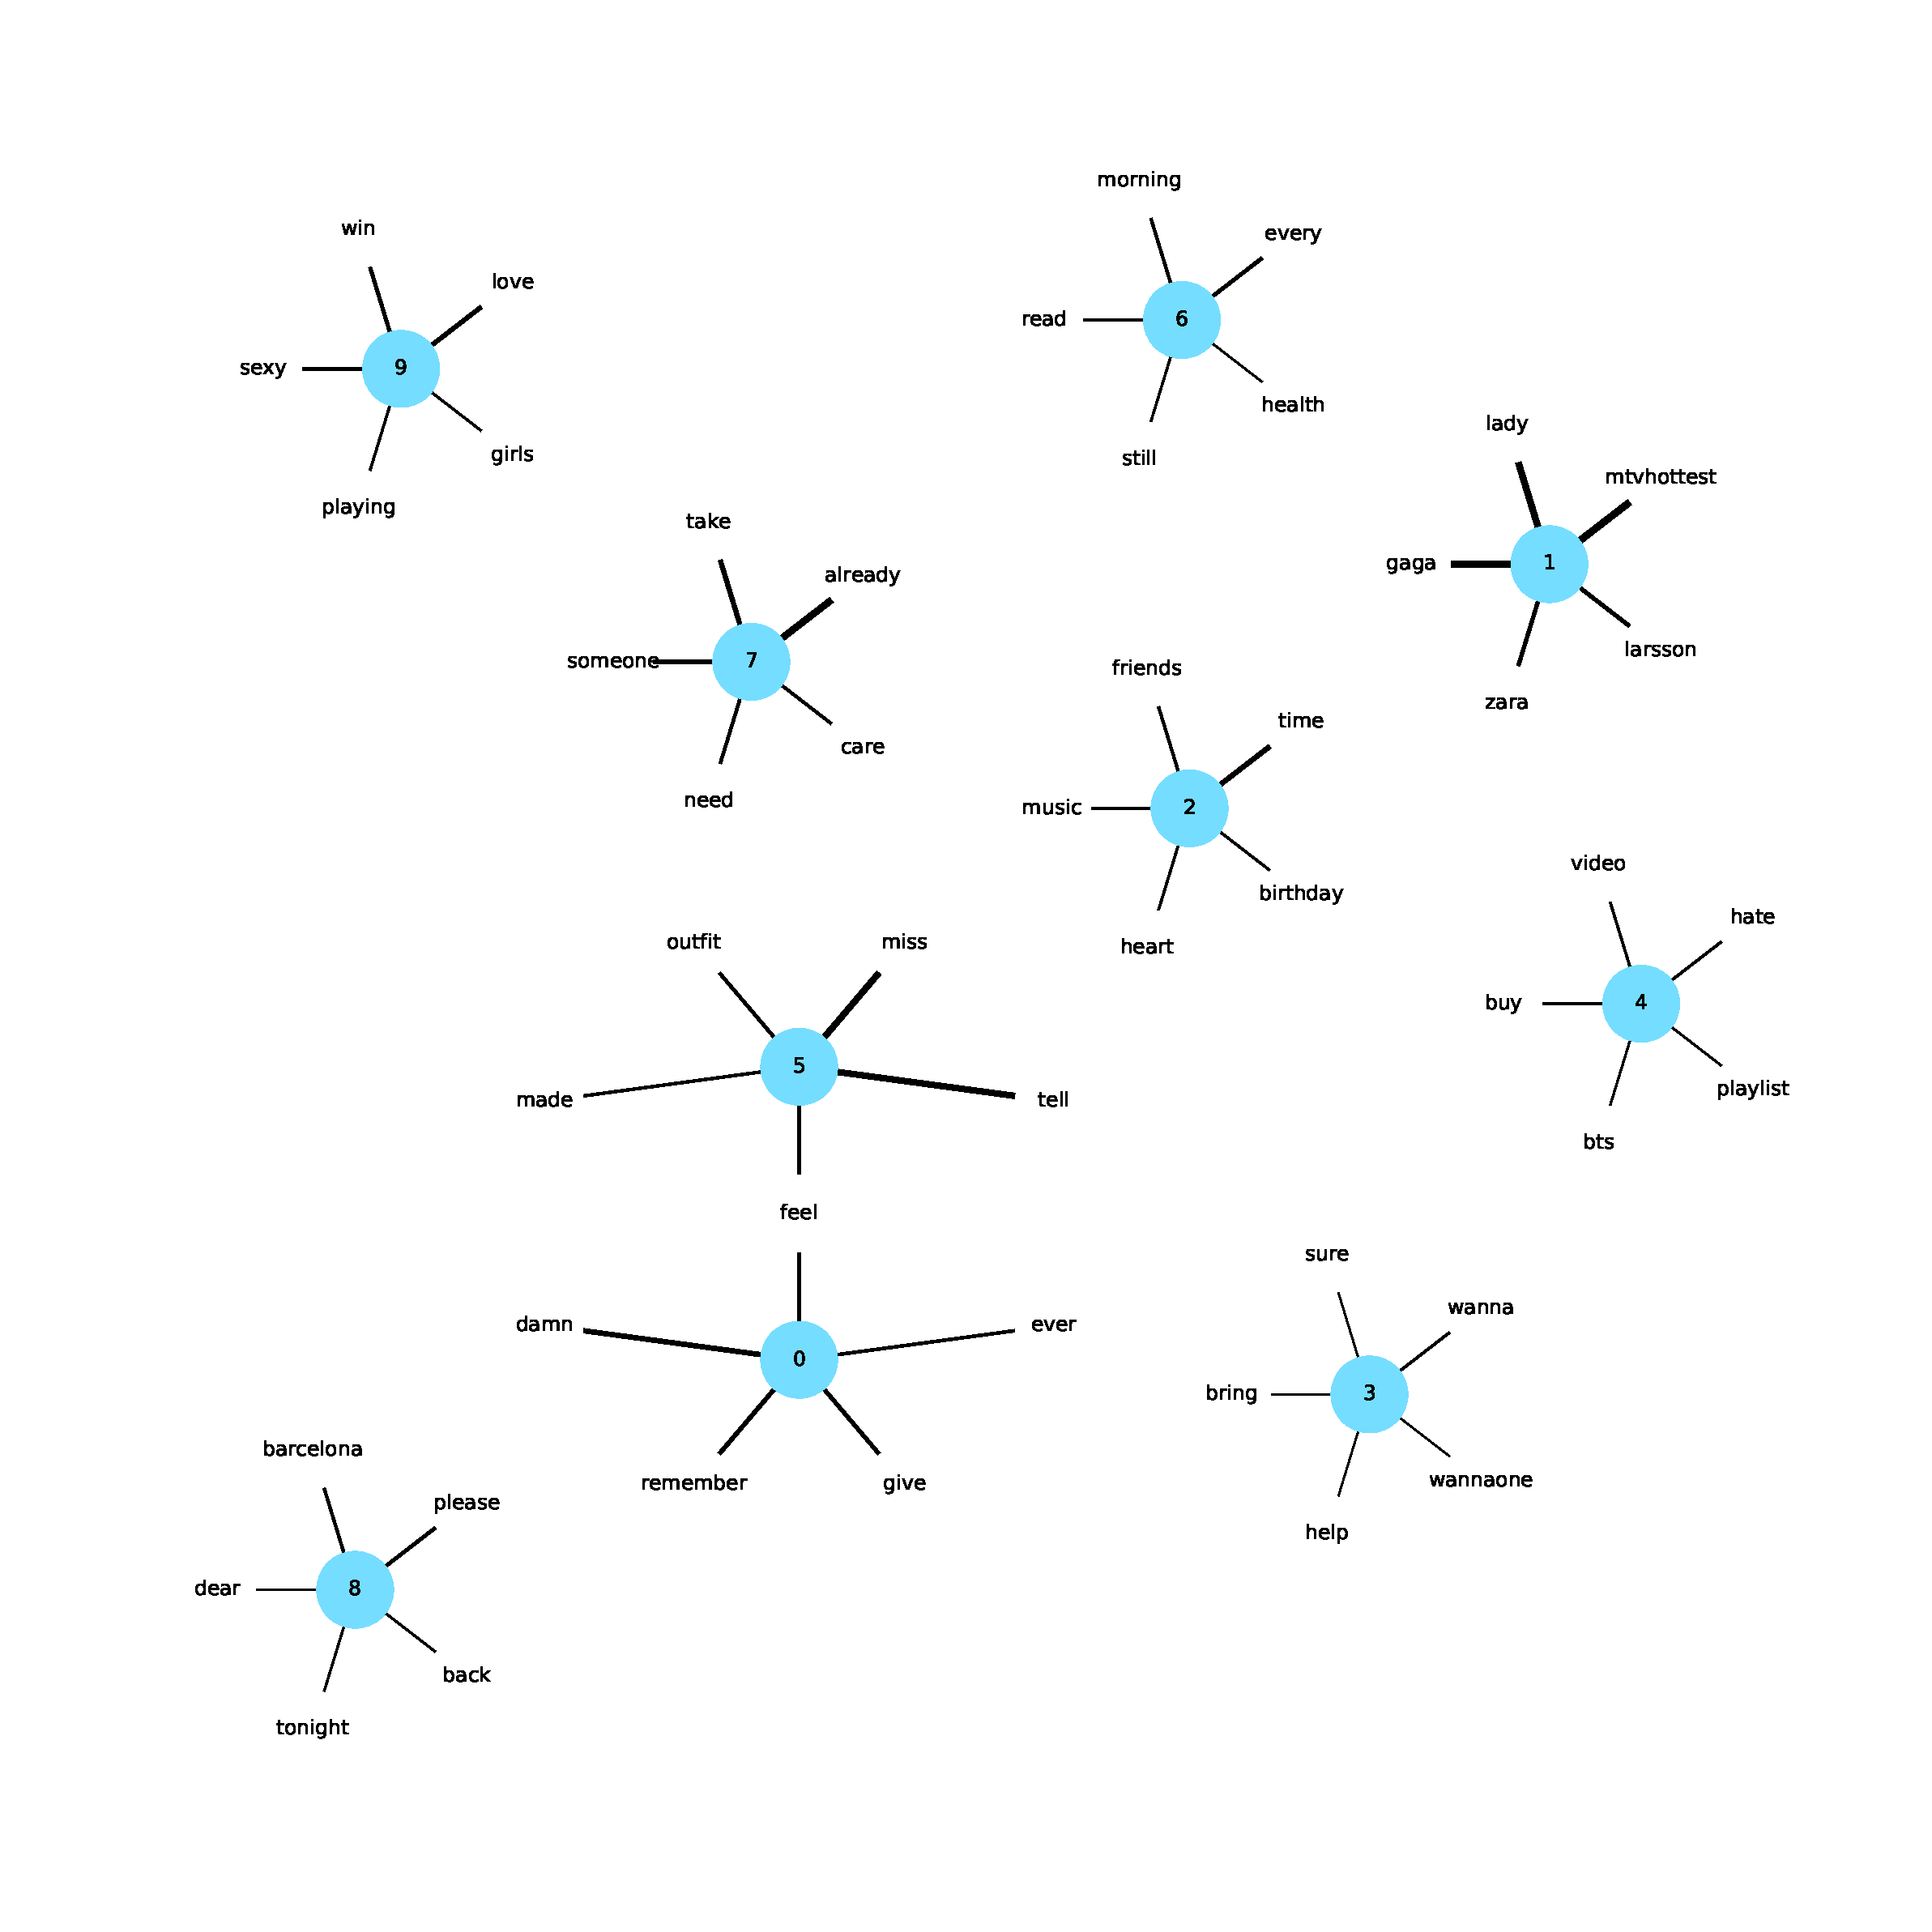
\includegraphics[width=\textwidth]{../figures/lda_network_graph.pdf}
\end{figure}

The training dataset was about equally distributed on the topic, as expected by the definition of LDA~\cite{Blei2003}.
This can be seen in~\ref{fig:sample_topic_distribution}.

\begin{figure}
    \centering
    \caption{Topic distribution of the LDA model trained on the sample dataset}
    \label{fig:sample_topic_distribution}
    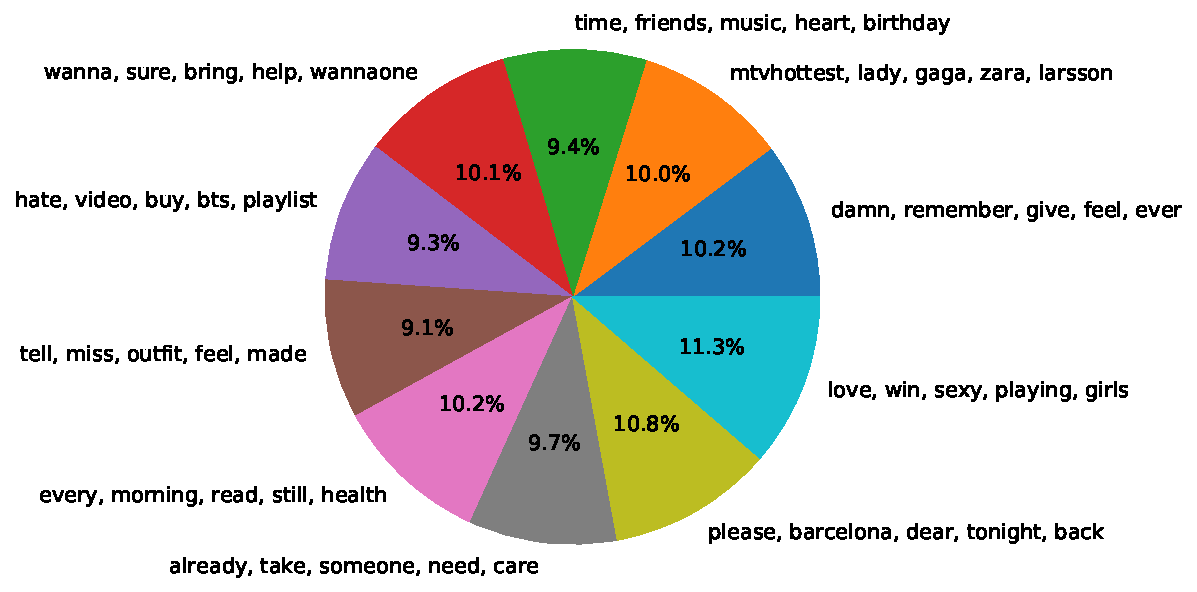
\includegraphics[width=\textwidth]{../figures/topic_distribution.pdf}
\end{figure}

\subsection{NMF}
\label{subsec:nmf}

NMF (\textbf{N}onnegative \textbf{M}atrix \textbf{F}actorization) is another active area of research in topic modeling.
It overcomes some of the shortcomings of LDA in terms of consistency across runs and empirical convergence,
since it is deterministic~\cite{Choo2013}.
It is also easier to adjust the model and incorporate feedback on the classification results in a semi-supervised approach,
making it a potentially more suitable solution for recommendation systems as described at the beginning of this chapter.
The output of the model is the same as the output of an LDA model: a term-wise representation of topics, even though the columns
do not necessarily sum up to 1.

The implementation of NMF in the scikit-learn library was used~\cite{scikitDocs}.
The number of components (the number of topics in this case) was set to 10 to ensure comparability with the LDA results.
Although several parameters were explored, the best results were accomplished with the default parameters.
The resulting network graph can be seen in~\ref{fig:nmf_network_graph}.

\begin{figure}
    \centering
    \caption{Network graph of the NMF topic model created from the stream sample dataset}
    \label{fig:nmf_network_graph}
    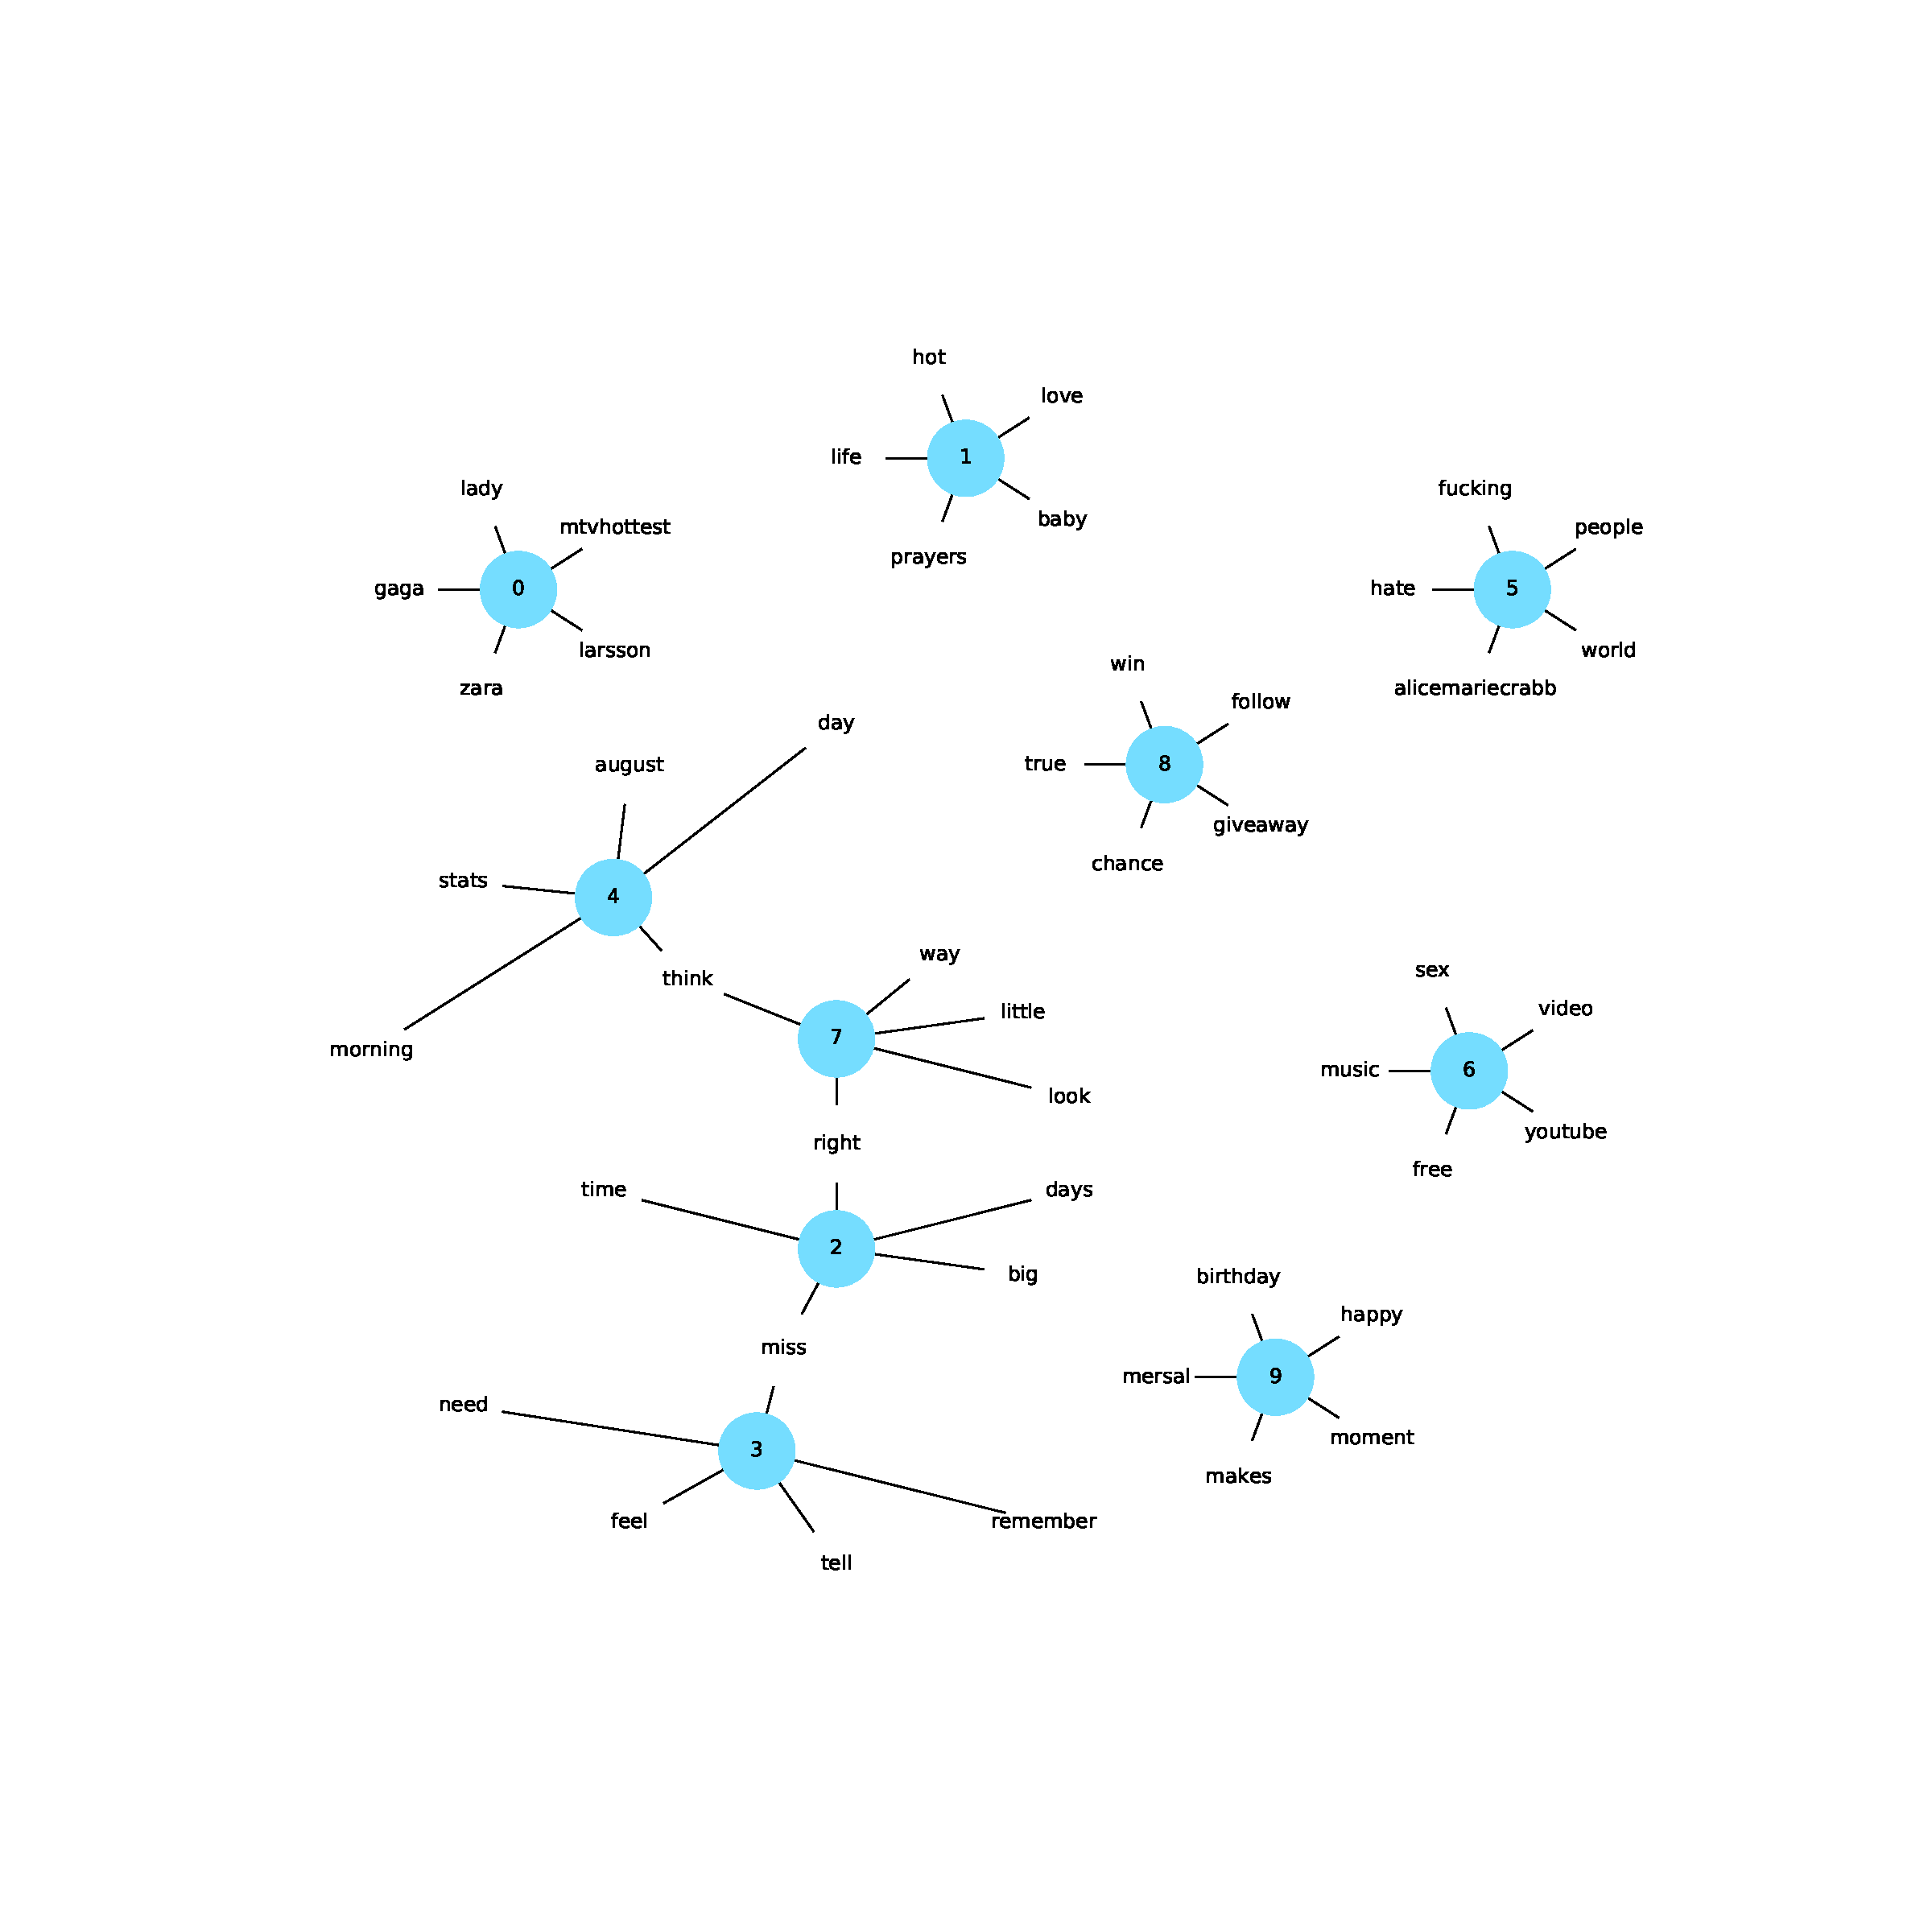
\includegraphics[width=\textwidth]{../figures/nmf_network_graph.pdf}
\end{figure}

\section{Results}
\label{sec:results}

Overall, the results that could be achieved with both methods were similar in terms of subjective descriptiveness of the top terms and amount of overlap.
There were even some equal topics, like topic number 6 in the LDA model and topic number 1 in the NMF model.
The advantages of NMF also do not apply to this usecase, therefore a decision was made in favor or LDA,
since it is the more mature method with more available research, implementations and tools like LDAvis, which can be used to comfortably
tune and explore models.
